\documentclass[letterpaper,12pt]{article}
\usepackage{tabularx} % extra features for tabular environment
\usepackage{amsmath}  % improve math presentation
\usepackage{graphicx} % takes care of graphic including machinery
\usepackage[margin=1in,letterpaper]{geometry} % decreases margins
\usepackage{wrapfig, blindtext}
\usepackage{graphicx}
\usepackage{placeins}
\usepackage{cite} % takes care of citations
\usepackage[final]{hyperref} % adds hyper links inside the generated pdf file
\hypersetup{
	colorlinks=true,       % false: boxed links; true: colored links
	linkcolor=blue,        % color of internal links
	citecolor=blue,        % color of links to bibliography
	filecolor=magenta,     % color of file links
urlcolor=blue}
%\FloatBarrier


\begin{document}
\title{}
\author{}
\date{}


\begin{center}
\textbf{Project 2: Advanced Lane Finding - Jack Wetherell} \\
\end{center}


\section{Introduction}
My computer vision (CV) pipeline takes a single frame image as an input, and returns the image with a green box indicating the area between the left and right lanes. It also displays the drift from the left of the centre of the lane, and the radius of curvature of the road measured in meters. This information can be used to steer the vehicle in order to keep centred on straight and curved roads.

This pipeline correctly annotates the given example images and project video, but has several shortcomings and possible improvements. I will now describe how I:
\begin{itemize}
\item Use calibration images to calibrate the camera to compute the camera matrix and distortion coefficients.
\item Implement a CV pipeline to annotate the lane lines for a series of test images.
\item Apply the CV pipeline to annotate the project video.
\item A discussion of the problems faces and how they were resolved, shortcomings and potential improvements. 
\end{itemize}
The project notebook \texttt{(advanced\_lane\_finding.ipynb)} contains the source code of this implementation, as well as the results. The output images of the pipeline are found in \texttt{output\_images/fig9.pdf}, and the final annotated video is \texttt{project\_video\_output.mp4}.


\section{Camera Calibration}
Before I created the main pipeline the camera was first calibrated. This was performed by implementing a calibration function that takes a list of chessboard calibration images, and returns a calibration dictionary containing the camera matrix and distribution coefficients. First, I define the coordinates of the chessboard in 3D space by defining the positions of the inner corners. Then I used openCV to find the chessboard corners in the calibration images and use these, in conjunction with the 3D points, to calibrate the camera by calculating the camera matrix and distortion coefficients. This is then used to create a undistortion function (details below). The figure below shows the undistortion function being applied to a sample of the calibration images.
\FloatBarrier
\begin{figure}
\centering
\makebox[\linewidth][c]{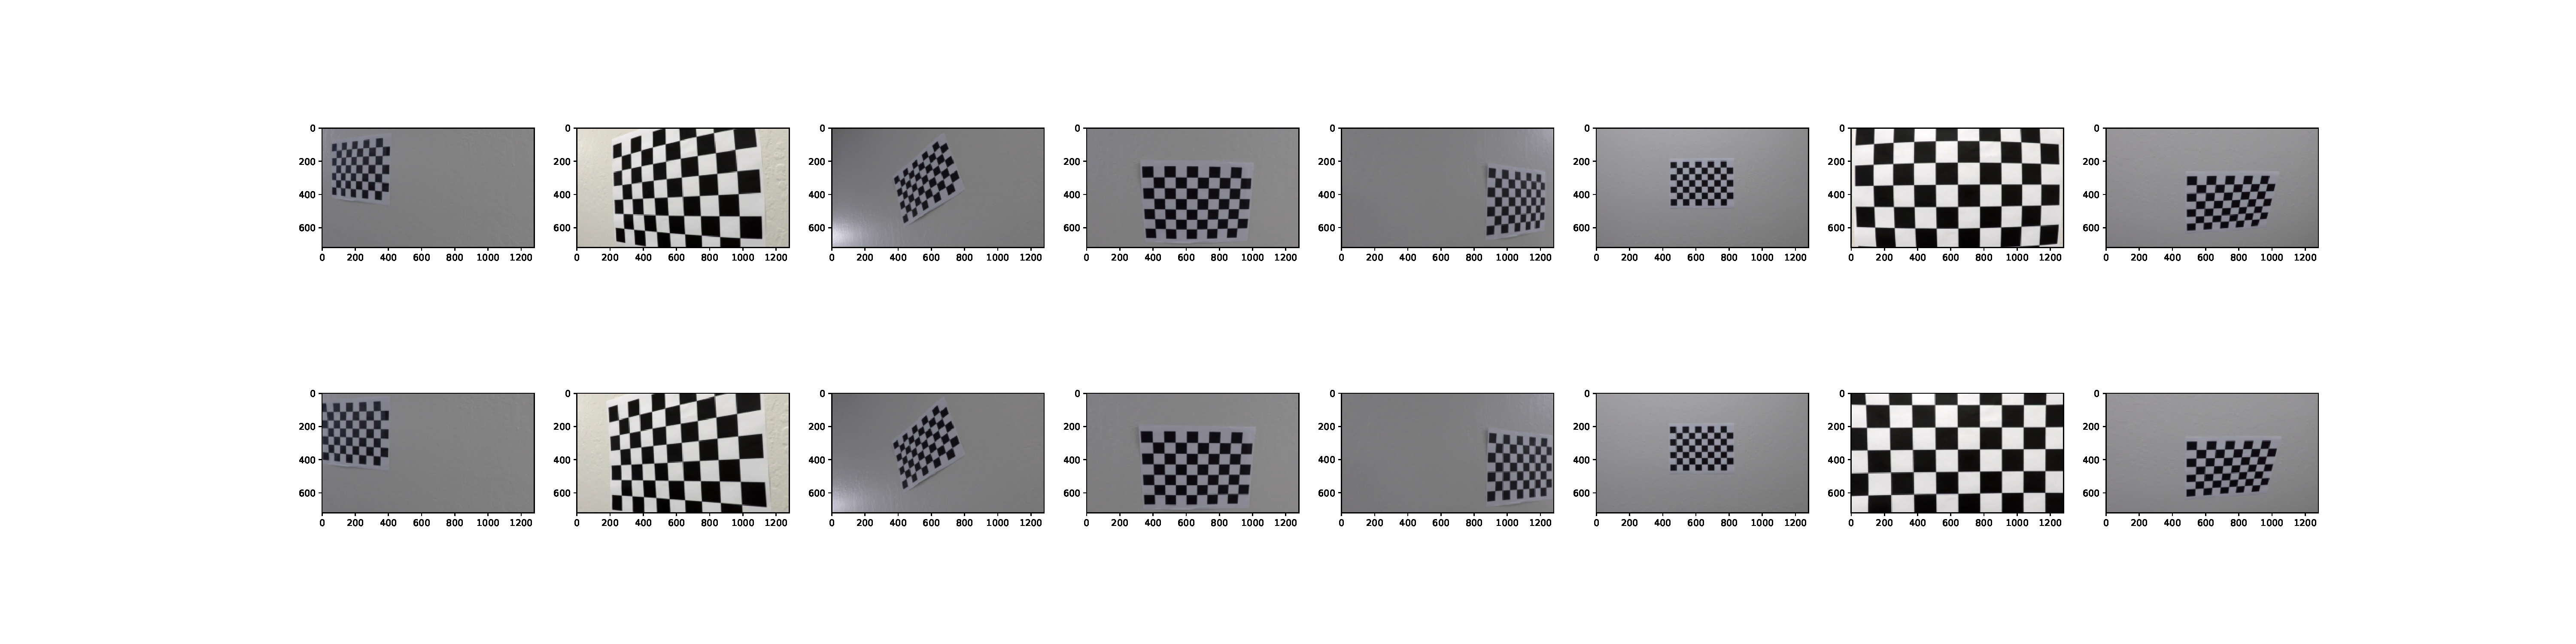
\includegraphics[scale=0.25]{output_images/cal_test.pdf}}
\end{figure}
\FloatBarrier


\section{Pipeline (Test Images)}
Here I summarise all the lane finding CV pipeline:
\begin{enumerate}
\item Distortion Correction
\item Perspective Transform
\item Gradient Thresholding
\item Color Space Thresholding
\item Histogram Peaks
\item Sliding Windows
\item Fit to the Lane Pixels
\item Search from Last Frame
\item Measuring Position and Curvature
\item Visualise the Result
\end{enumerate}
Each of these is represented as a function in the project notebook, with doc strings and comments to provide documentation. At each stage I plot the results for all of the test images. The files \texttt{output\_images/fig*.pdf} contain all of the figures showing each stage of the pipeline. Here I will go through the method of each stage, showing the test images at each stage as they pass though the pipeline.
\newpage
\subsection{Distortion Correction}
Here I use the camera calibration values computed in the previous section to define a function to undistort a given image. This simply involved passing the camera matrix and distorting coefficients along with the image into the openCV routine. This correctly removes the camera distortion in the test images. The figure below shows this stage of the pipeline applied to the test images. The top row shows the original images, and the bottom shows the undistorted images. 
\FloatBarrier
\begin{figure}
\centering
\makebox[\linewidth][c]{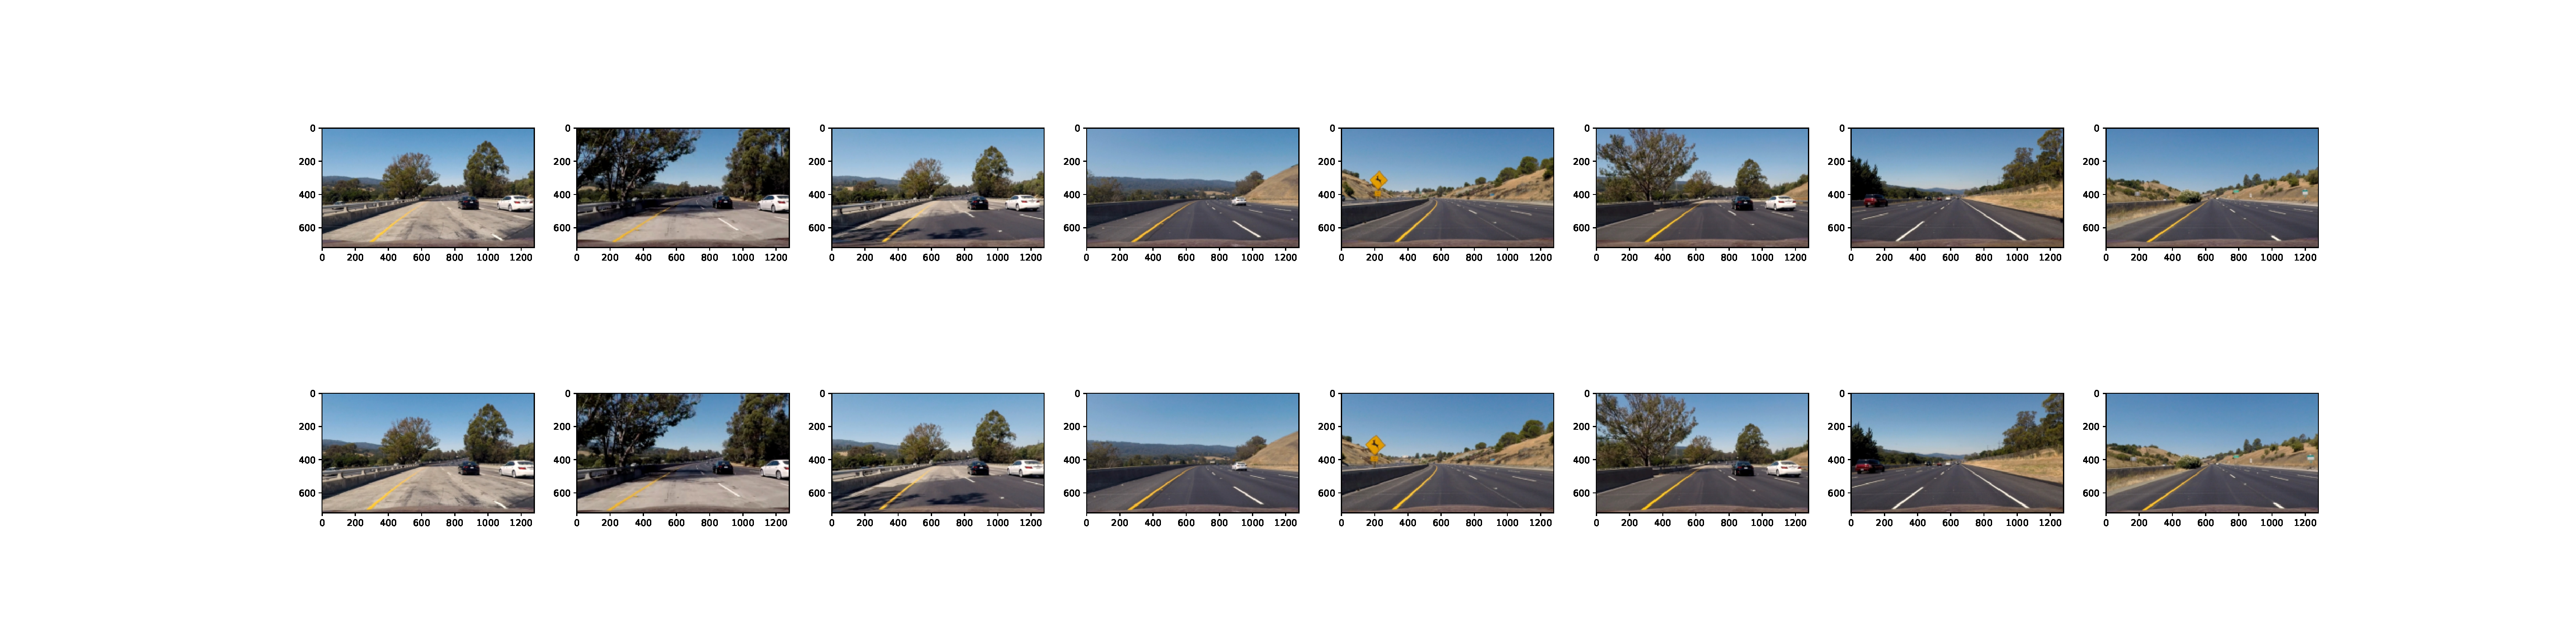
\includegraphics[scale=0.25]{output_images/fig1.pdf}}
\end{figure}
\FloatBarrier
\subsection{Perspective Transform}
The next stage is to apply a perspective transform to the images. This shifts the perspective from the view down the road, to the birds eye view from the top of the road. I chose the source and destination points to be [[80, 650], [540, 460], [740, 460], [1200, 650]] and [[20, 700], [20, 20], [1260, 20], [1260, 700]] respectively. I adjusted these values in order to achieve parallel exactly straight lines in the last two test images, using these as the ground truth. I also ensured all curved lines were also parallel. I did this stage before the later thresholding stages as it allowed me to more clearly check the perspective transform was working correctly in the two ground truth cases. The result of this stage of the pipeline is shown below.
\FloatBarrier
\begin{figure}
\centering
\makebox[\linewidth][c]{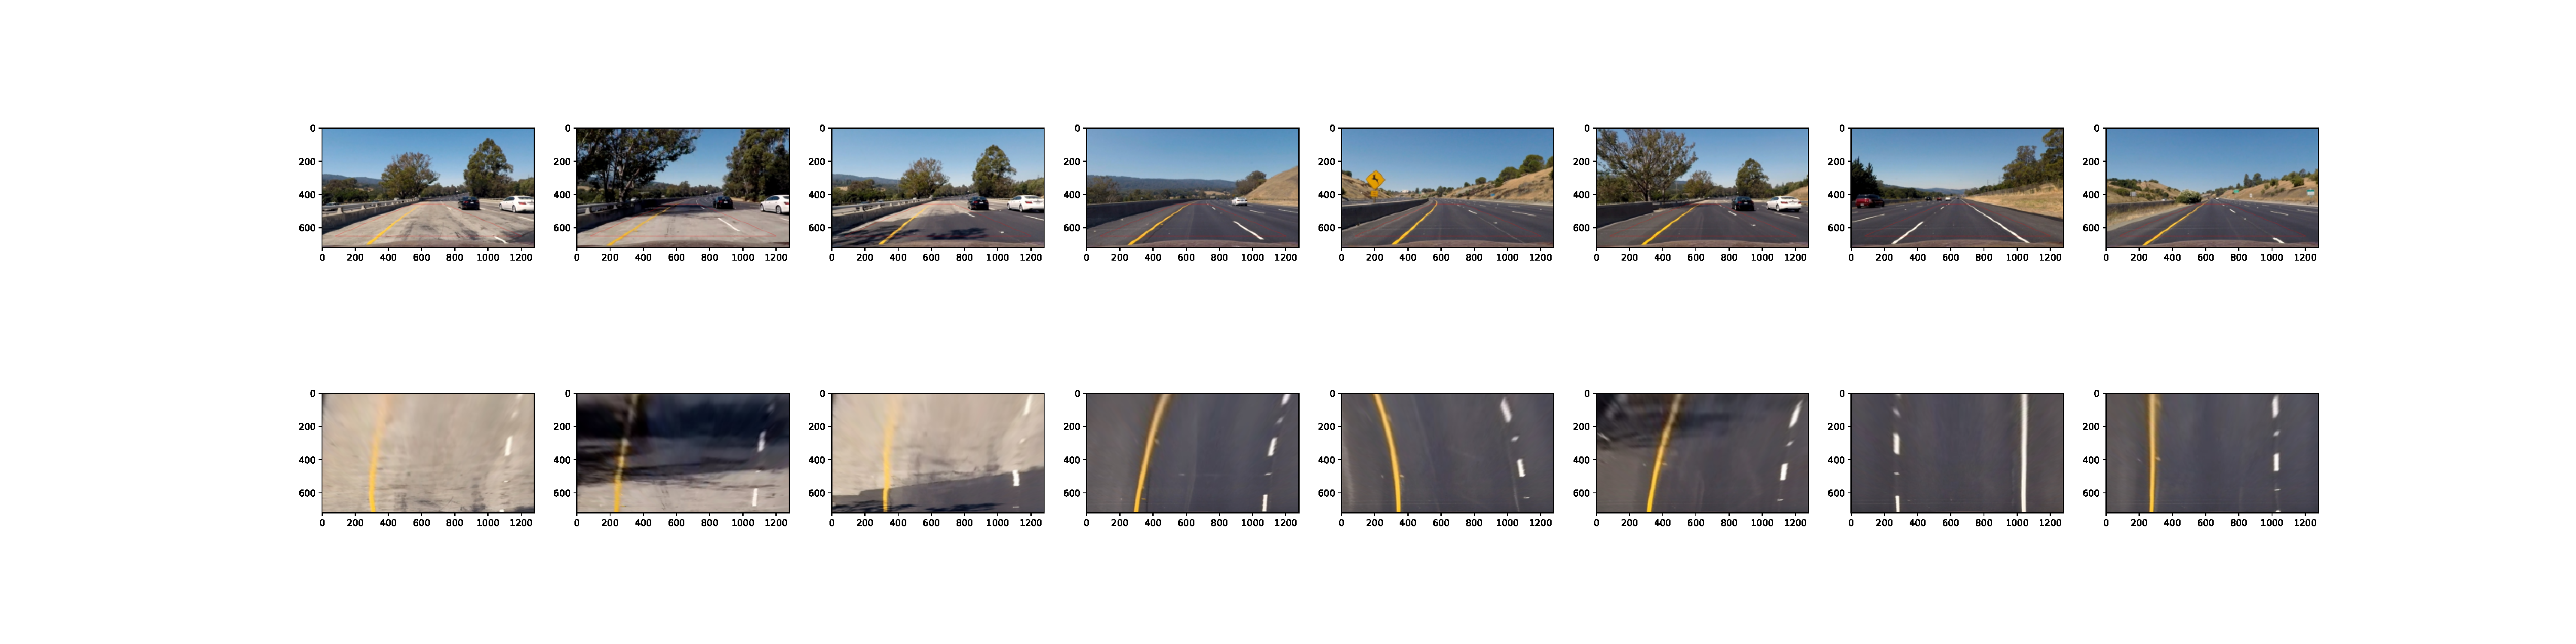
\includegraphics[scale=0.25]{output_images/fig2.pdf}}
\end{figure}
\FloatBarrier
\subsection{Gradient Thresholding}
The next stage is to apply a gradient threshold to the warped images. I chose to take the logical OR of the images thresholded by each of the 4 possible gradient based thresholds (x, y, magnitude and gradient). The values of each of these is as follows:
\begin{enumerate}
\item x - threshold=(20, 255)
\item y - threshold=(250, 255)
\item magnitude - threshold=(250, 255)
\item direction - threshold=(0.2, 0.4)
\end{enumerate}
I adjusted the values so that each of the 4 types each found certain parts of the lane. Taking the logical OR then `merged` them together to find as much of the lane as possible. The figure below shows the application of this stage of the pipeline.
\FloatBarrier
\begin{figure}
\centering
\makebox[\linewidth][c]{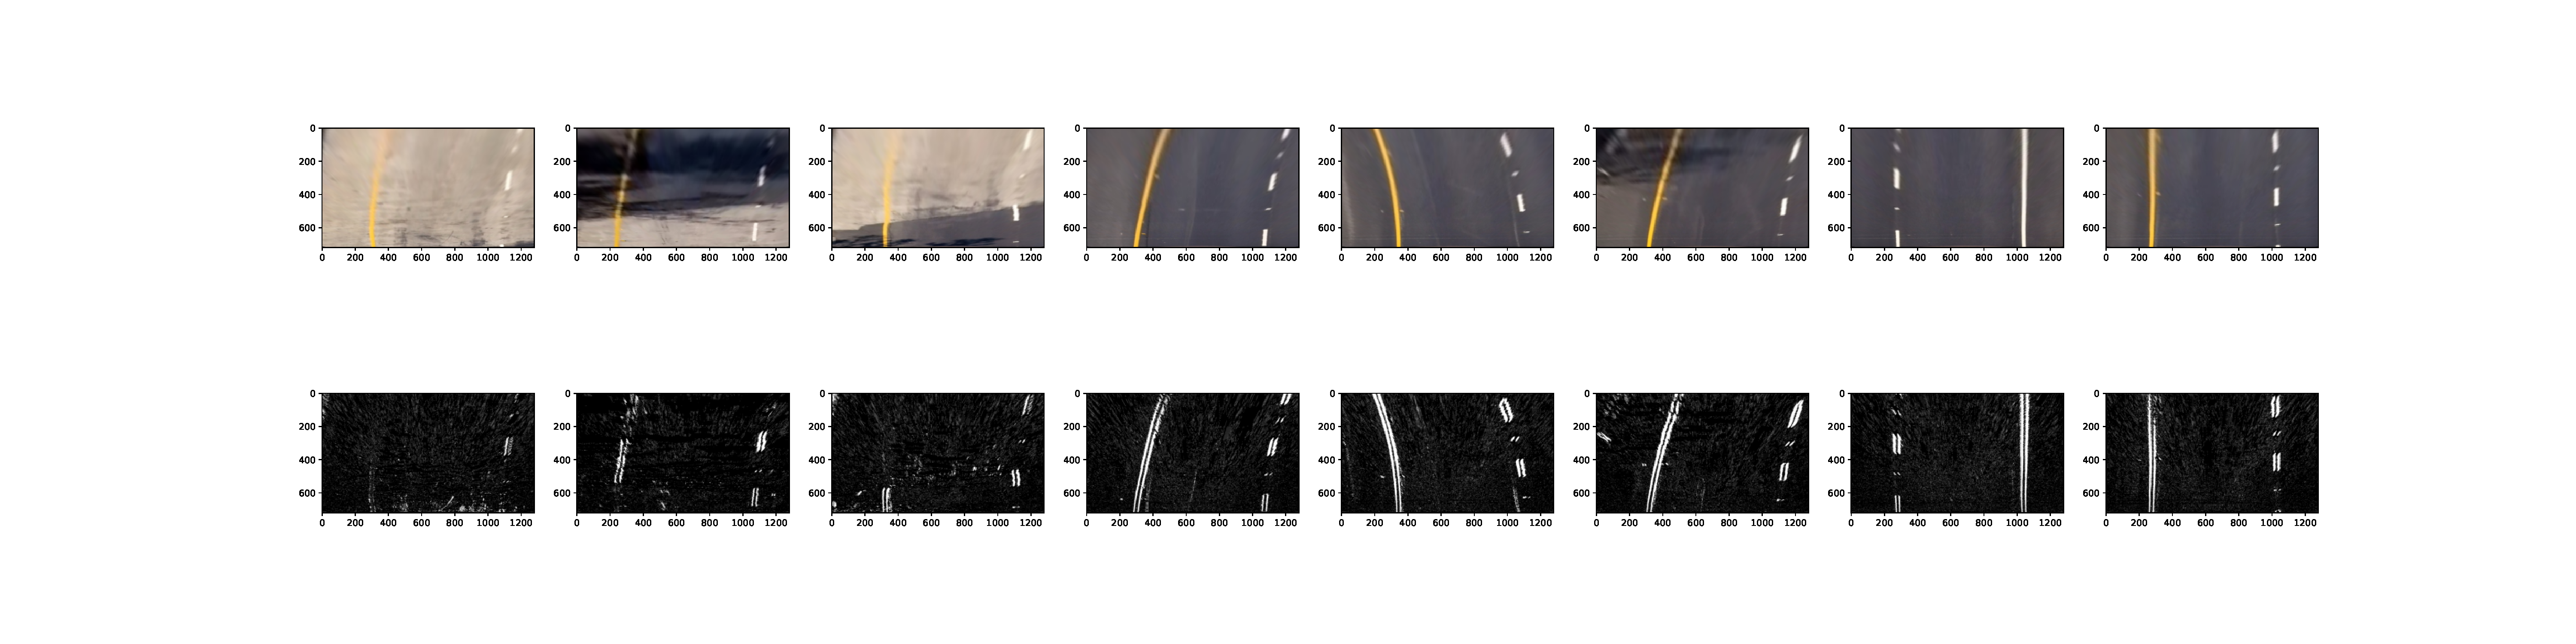
\includegraphics[scale=0.25]{output_images/fig3.pdf}}
\end{figure}
\FloatBarrier
\subsection{Color Space Thresholding}
The next stage is to separately apply various color thresholds the the warped image, and then merge this with the previous step by taking the logical OR of the total gradient thresholding, and each of the color thresholds individually. This followed the same reasoning: By tuning each of the color channel thresholds to identify different part of the lane, minimising false positives, this allows each of the channels to identify different parts of the lane, that are all merged at the end with an OR operation. 

I first converted from RGB to HLS color space, and then applied the following thresholds to each color channel:
The values of each of these is as follows:
\begin{enumerate}
\item H - threshold=(20, 200)
\item L - threshold=(210, 255)
\item S - threshold=(0.0, 1.0)
\end{enumerate}
The result of the total thresholding (gradient + color) is shown in the figure below:
\FloatBarrier
\begin{figure}
\centering
\makebox[\linewidth][c]{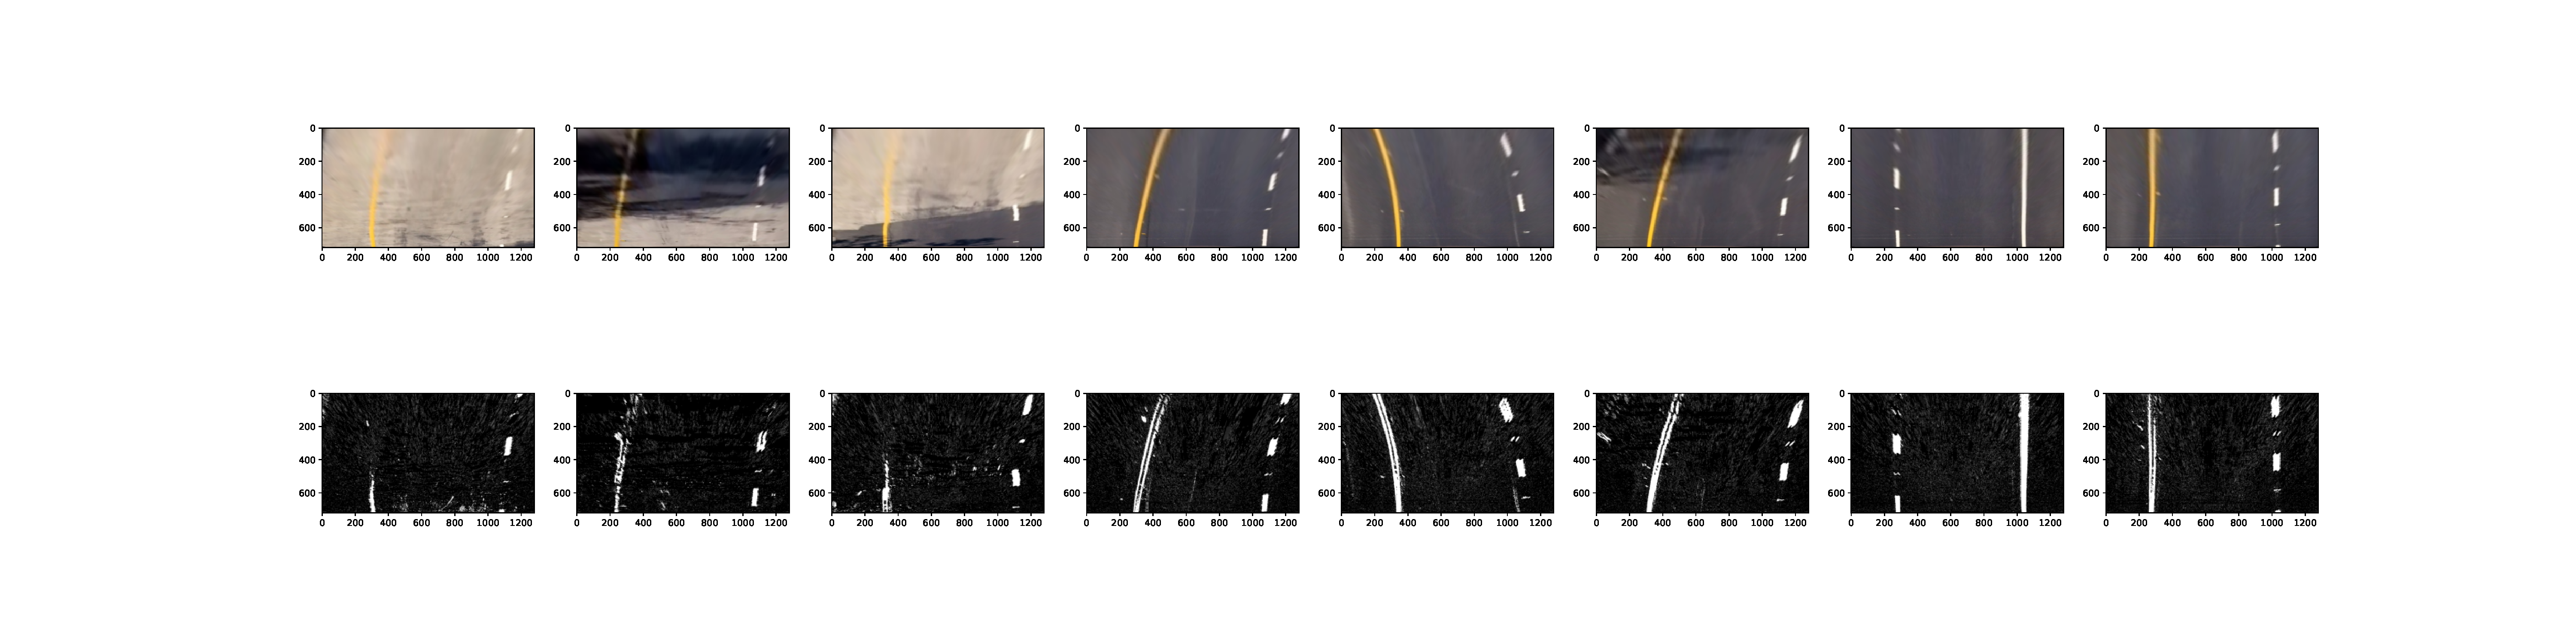
\includegraphics[scale=0.25]{output_images/fig4.pdf}}
\end{figure}
\FloatBarrier
\subsection{Histogram Peaks}
In order to locate the positions of the lanes in the warped and thresholded image I used a histogram to count how many lane line pixels are present in each row of the bottom half of the image, and used the magnitude of this hisogram to determine the lane locations. This is used to both locate the positions of the lanes, and to determine the initial position for the sliding window method described in the next subsection. The histograms of each of the test images is shown in the figure below:
\FloatBarrier
\begin{figure}
\centering
\makebox[\linewidth][c]{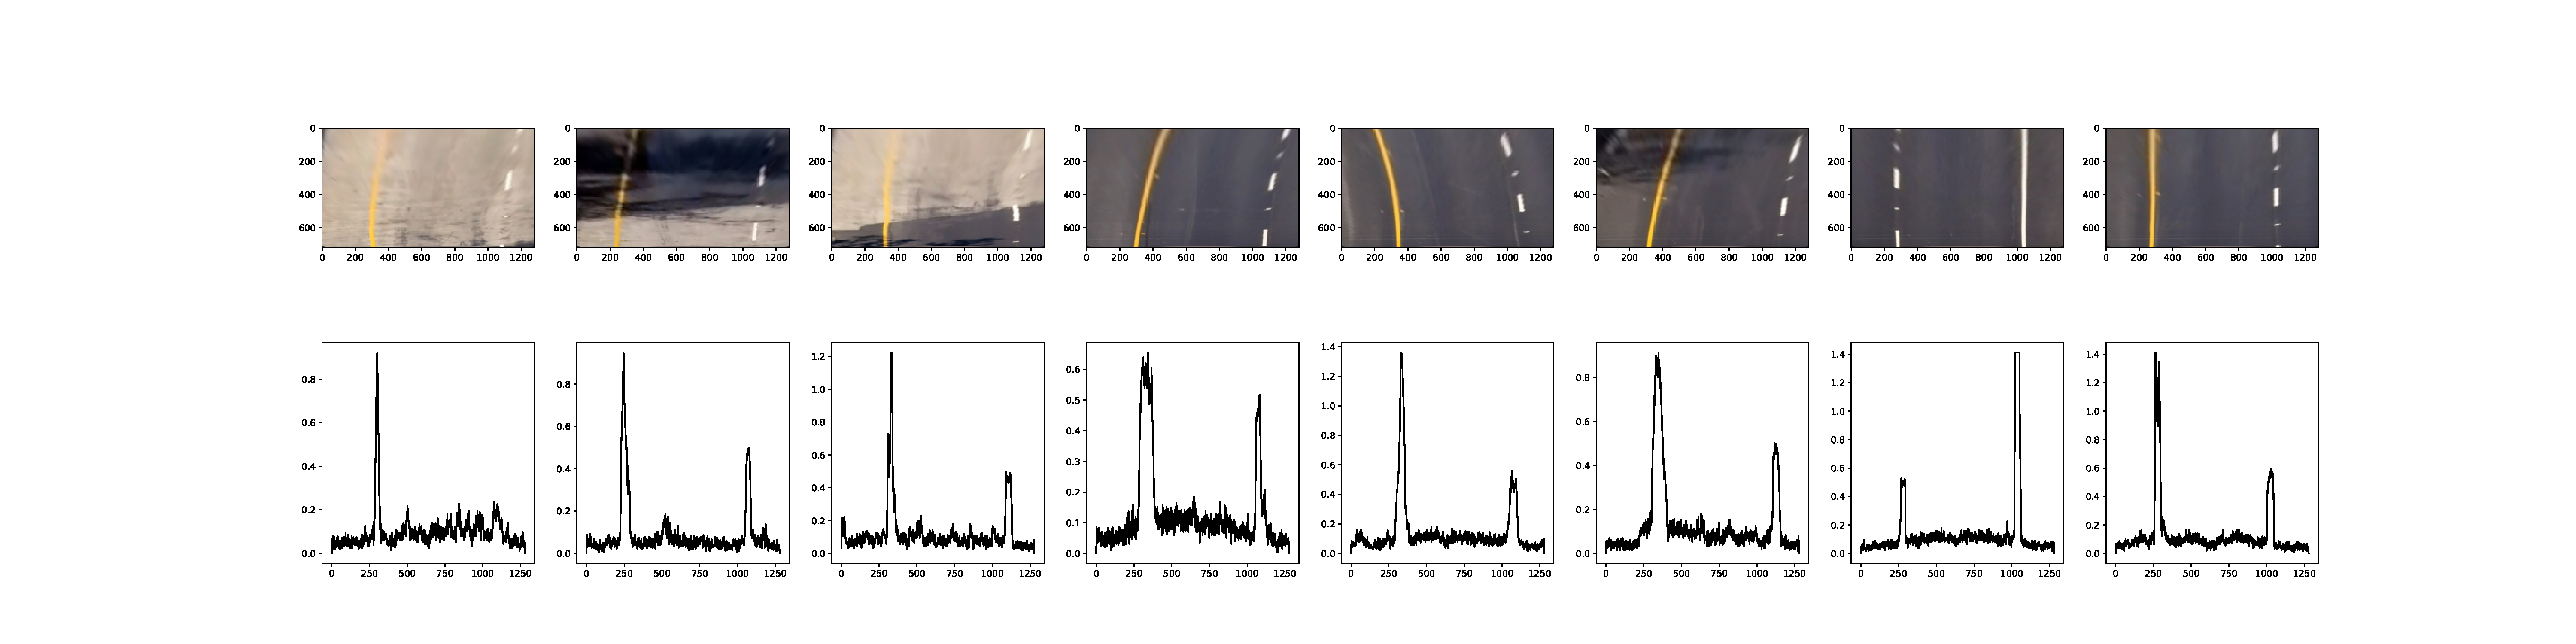
\includegraphics[scale=0.25]{output_images/fig5.pdf}}
\end{figure}
\FloatBarrier
\subsection{Sliding Windows}
The next stage is to use the histogram peaks as the initial location of a sliding window algorithm.  This method first finds the positions of the lanes using the peaks of the left and right distributions in the histogram. These are used as the initial locations of the sliding windows at the bottom of the image. The layer above is then scanned over with a sliding window to determine the non-zero pixels in the region. If a sufficient number of pixels is detected the window locks in place, and we move onto the layer above. This is repeated until the top of the image is reached. Only the lane line pixels within the sliding windows are passed forward to the next stage of the pipeline. The figure below shows an illustration of the sliding window method applied to the test imaged:
\FloatBarrier
\begin{figure}
\centering
\makebox[\linewidth][c]{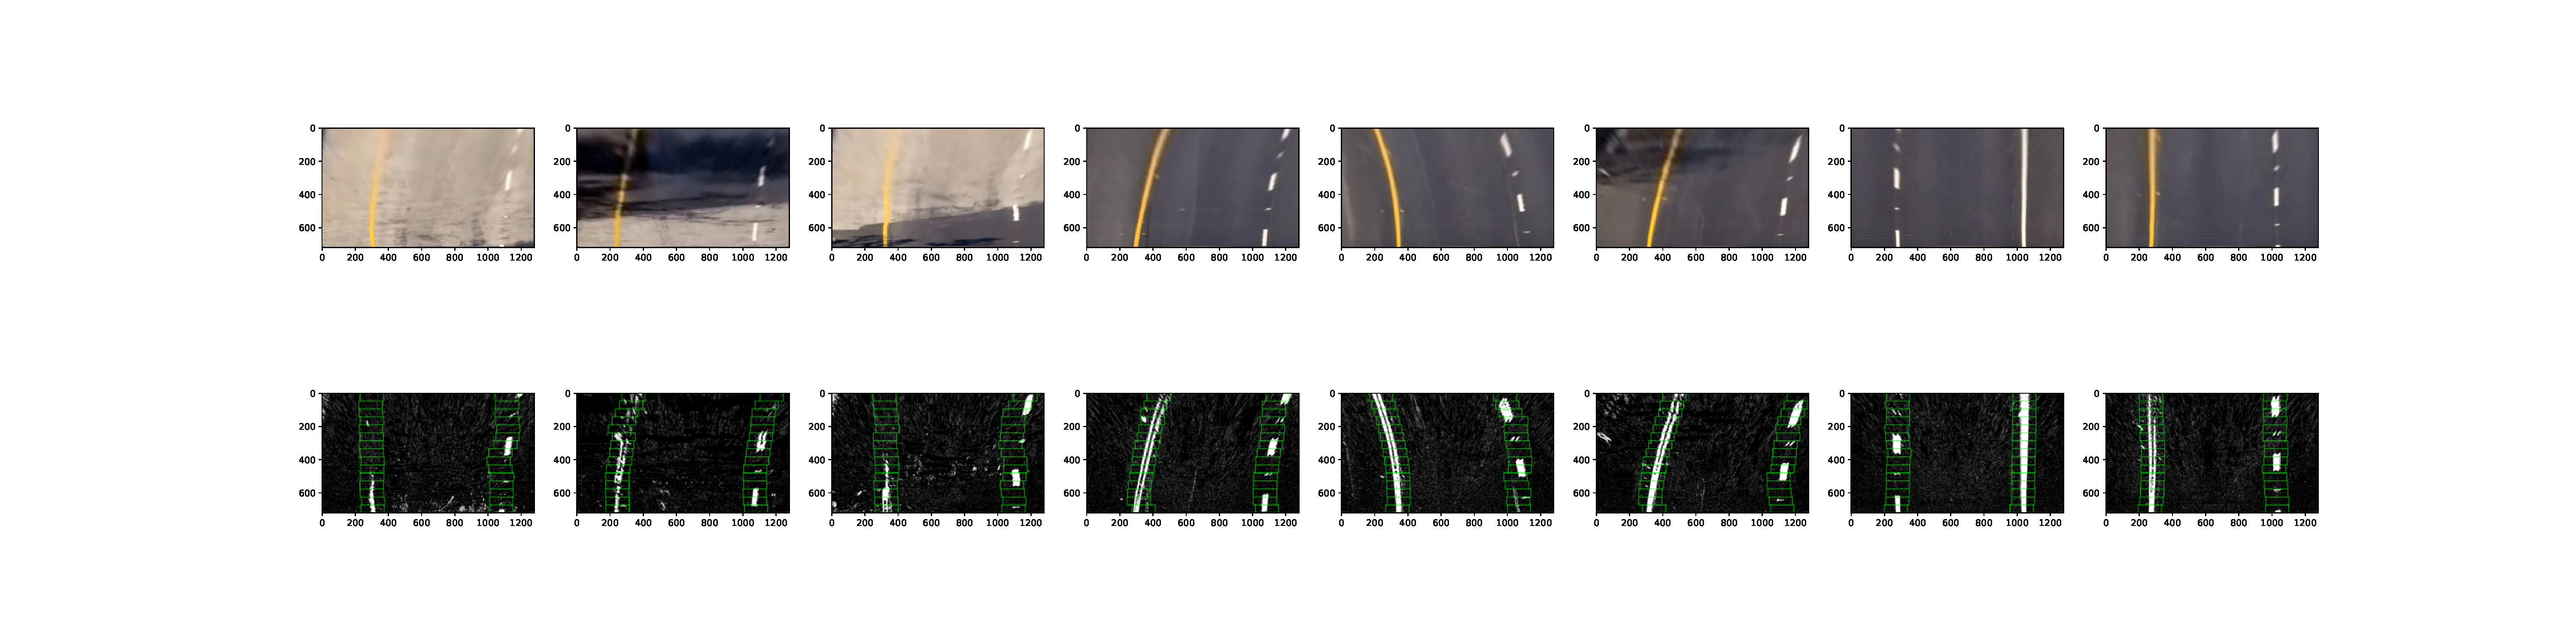
\includegraphics[scale=0.25]{output_images/fig6.pdf}}
\end{figure}
\FloatBarrier
\subsection{Fit to the Lane Pixels}
The next stage is to take the lane line pixels as determined by the previous stage, and perform a second order polynomial fit to the left and right lane line pixels separately. This second order polynomial is resistant to over fitting but allows for the expected amount of curvature present in road lane lines. The figure below shows these lane lines being drawn on the test images.
\FloatBarrier
\begin{figure}
\centering
\makebox[\linewidth][c]{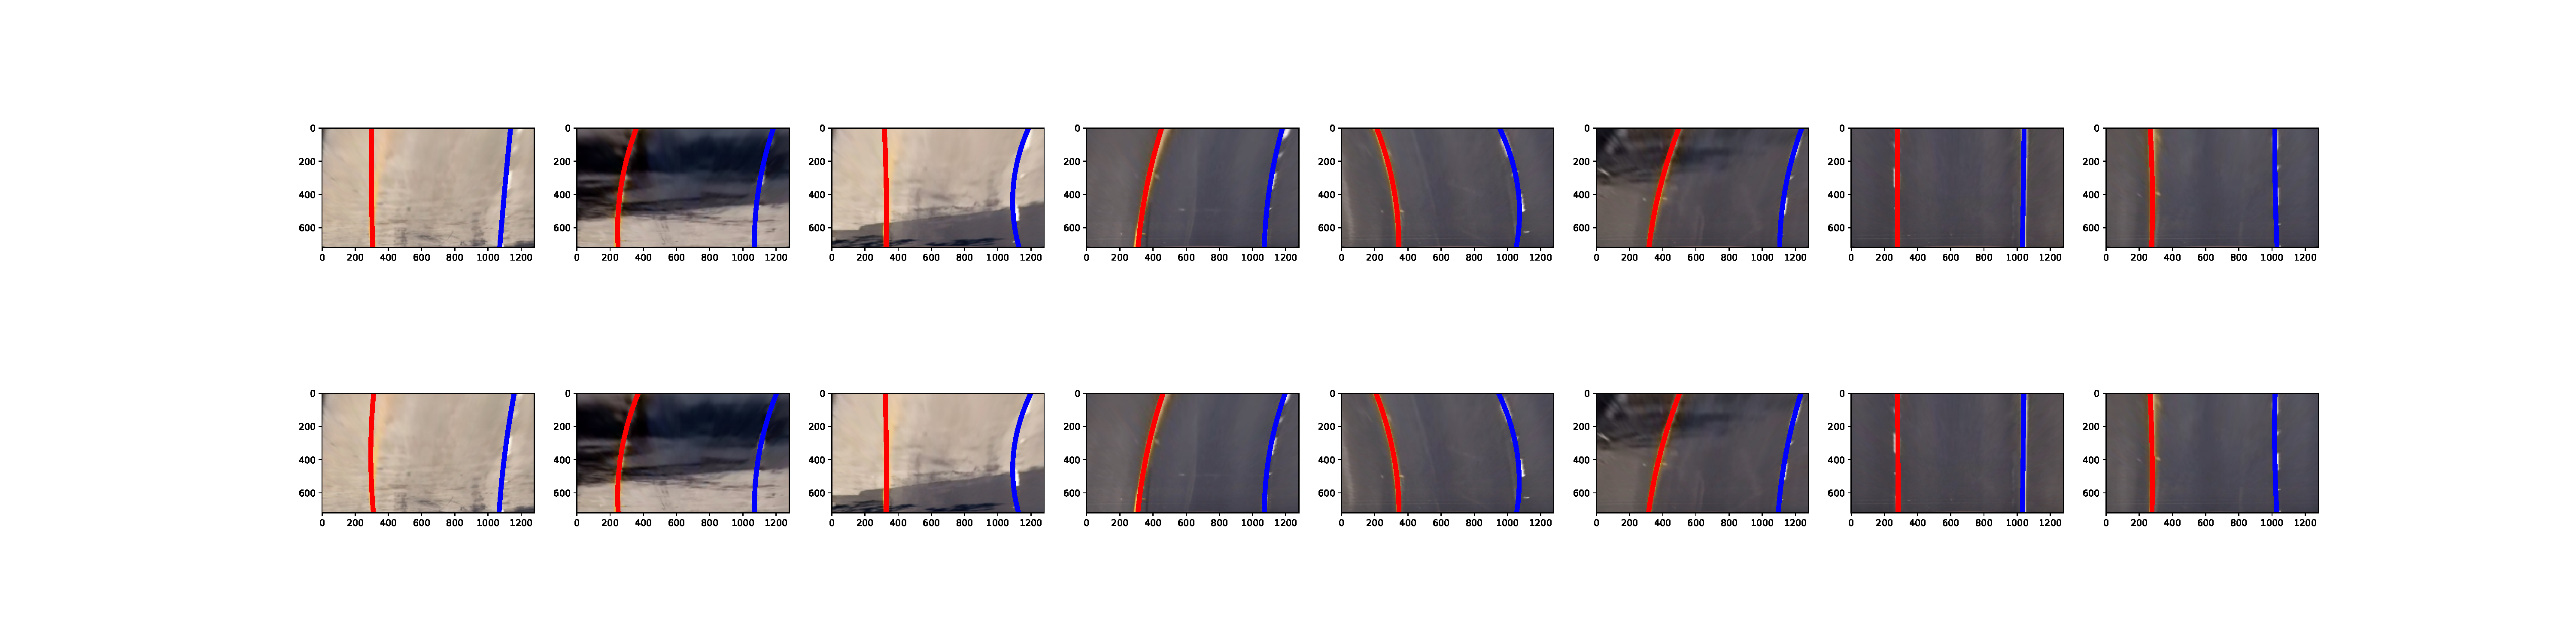
\includegraphics[scale=0.25]{output_images/fig7.pdf}}
\end{figure}
\FloatBarrier
\subsection{Search from Last Frame}
In each frame of a video stream, I do not have to begin the search from scratch each time, this is because the lanes will only move an infinitesimal amount as we move from frame to frame. The next stage in the pipeline is therefore to define a function that allows us to use the polynomial fit parameters I found in the last frame to inform the search region in the current frame. This cannot be applied to the test images as they are not sequential, but in the final video stream, only every 5 frames the polynomials are recalculated from scratch, this yields improved performance of the CV pipeline. 
\subsection{Measuring Position and Curvature}
The next stage is to use the polynomial fit parameters and the histograms to determine the radius of road curvature and lane positions respectively. I use the peaks of the histograms as the positions of the lanes, and apply the formulae for the curvature of radius to the found polynomial fit parameters. I take the difference in the lane line positions to calculate the drift from the centre lane, and take the average of the left and right lane curvatures to yield the road curvature. These will both be written onto the final video output.
\subsection{Visualise the Result}
In the final stage of the pipeline, I use the found left and right lane fits to draw a green box on the road, who's left and right edges and the found left and right lane lines respectively. I also add text to the image showing the drift to the left of centre and radius of road curvature. The figure below shows the final results of the pipeline being applied to the test images.
\FloatBarrier
\begin{figure}
\centering
\makebox[\linewidth][c]{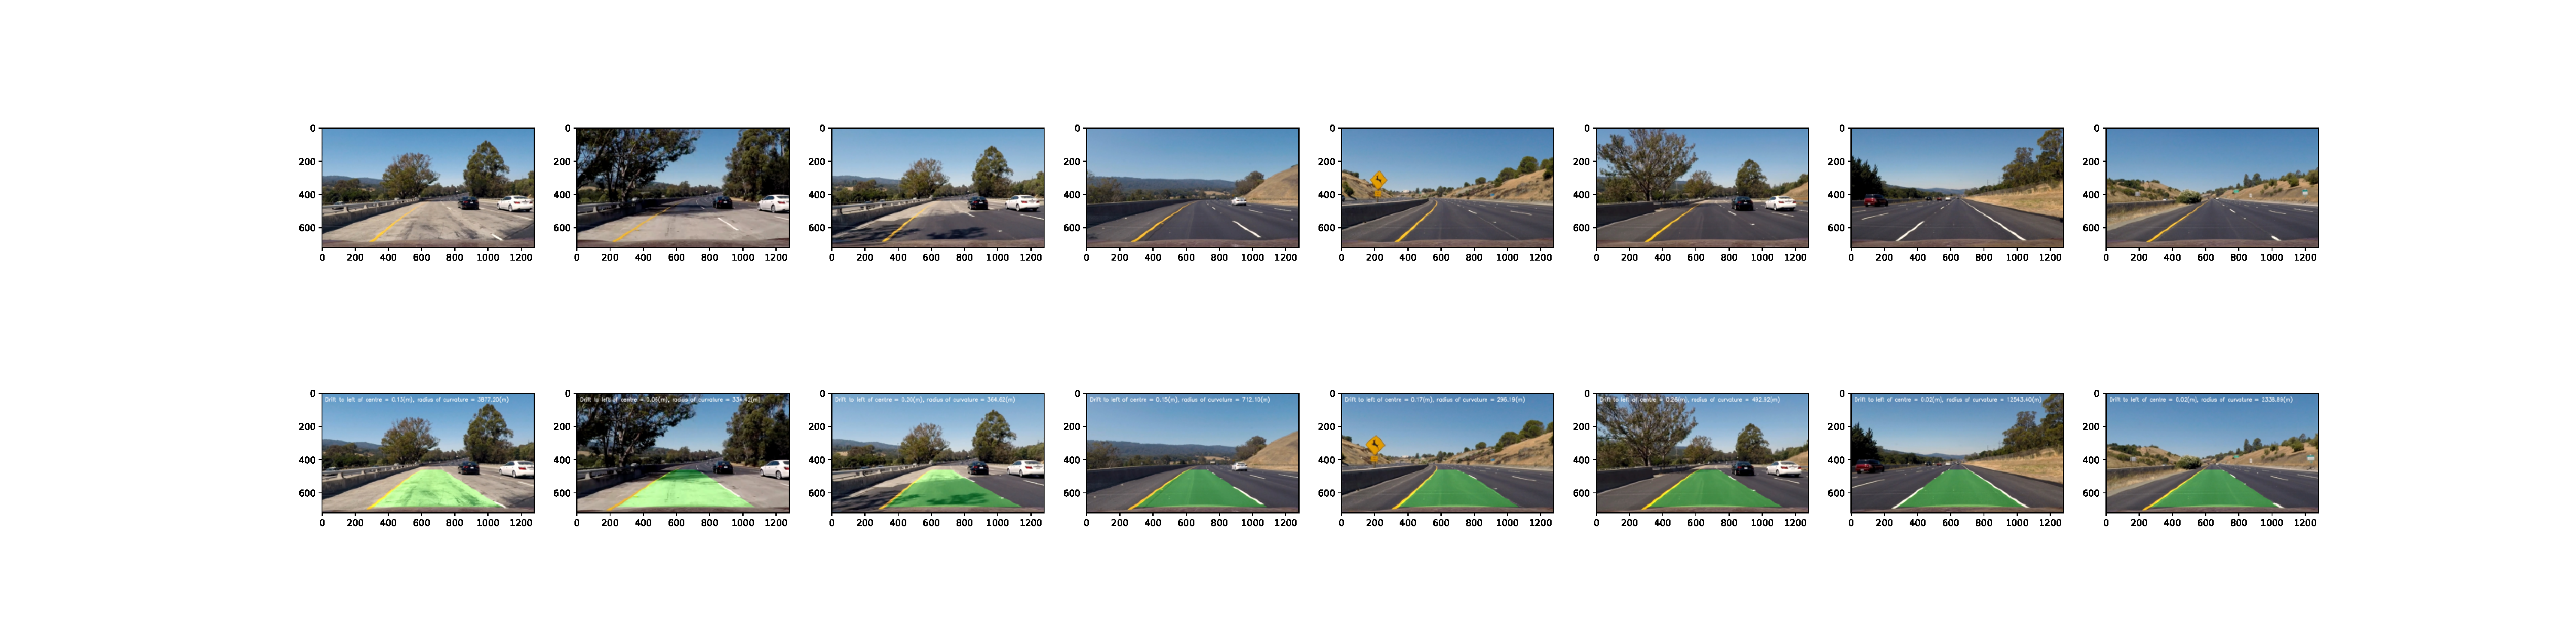
\includegraphics[scale=0.25]{output_images/fig9.pdf}}
\end{figure}
\FloatBarrier


\section{Pipeline (Video)}
This pipeline was then applied to the project video. The performed very well and smoothly for all but 3 outlier frames. This video is in the project directory as \texttt{project\_video\_output\_outliers.mp4}. In order to ensure the pipeline is resilient to these outliers, I added a time dependent error resistance. I chose a representative parameter from one of the fits that illustrate the outliers by jumping suddenly. In the figure below in red, I show the gradient of this parameter as a function of the frame. As can be seen, this allows the definition of a threshold (+/- 100) that defines the three outlier frames. When an outlier frame is detected once the gradient of the representative parameter jumps out of the threshold the pipeline rolls back to the fit from the previous frame. This ensures that no unrealistic sudden jumps in the fits can occur. In the figure below in black I show the value of the gradient of the representative parameter is corrected by the error resistance. This produces a video that shows the lanes correctly identified in all frames, with no outliers. This corrected video is in the project directory as \texttt{project\_video\_output.mp4}. 
\FloatBarrier
\begin{figure}
\centering
\makebox[\linewidth][c]{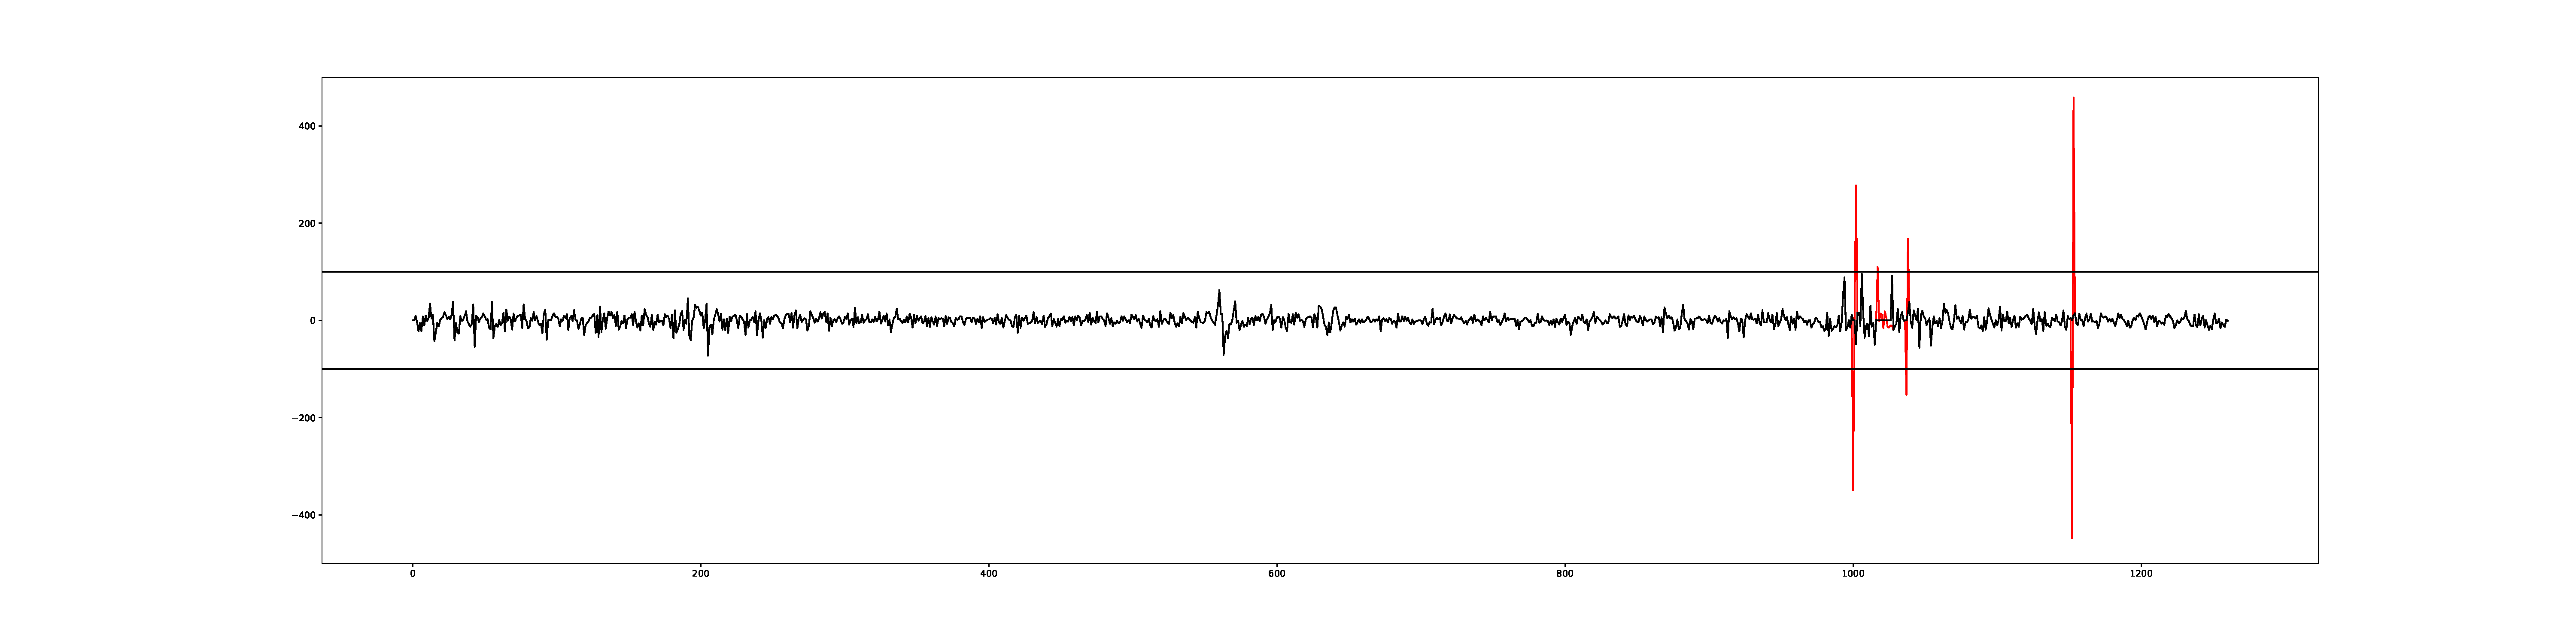
\includegraphics[scale=0.25]{output_images/outliers2.pdf}}
\end{figure}
\FloatBarrier


\section{Discussion}
The main issue faced during the creation of this CV pipeline was outliers appearing in the final video stream. This was fixed by recognising the large sudden single frame jumps are not possible, and so developing the time dependent outlier resistance as described above solved this issue and resulted in a stable output video annotation. 
I have identified the following shortcomings in the CV pipeline:
\begin{enumerate}
\item The hyper parameters are only trained to work on this particular road type as show in the test images. Roads substantially different (including weather effects) are not guaranteed to produce clean lane lanes.
\item It does not fully utilise the fact that lane footage will always be smooth (no sudden jumps), only discarding outliers based on outlier detection.
\item Due to the left and right lane separation stage via the histograms, this would not be effective during the transition of lane changing.
\end{enumerate}
I suggest the following improvements to the pipeline, for each of the shortcomings discussed above:
\begin{enumerate}
\item These hyper-parameters could be tuned to a large range of testing images, with ground truths pre-applied. This could be done via something simple like grid-search, or more robust like n evolutionary search algorithm. 
\item This could be rectified by adding a more sophisticated extrapolation of previous frames using a configured weighted average of previous similar frames.
\item This could be solved by using extrapolation based on earlier frames in the video, as the transition over the lane occurs. 
\end{enumerate}


\end{document}